\section{The mobile application}
\subsection{User interface and flow of the user interaction}

We will now go through the application, by playing a level 2 scenario. We will discuss the game elements, the user interface, the technologies which are used. Whenever it is necessary to clarify we will also go deeper into the implementation.

The application is written in JavaScript, using the mobile application framework React Native \parencite{ReactNative}. The intention of using such a framework, is in the future to make iOS and UWP versions, without having to rewrite the entire application. As React Native uses the React web framework \parencite{React}, JavaScript, and that we can decouple some of the data management logic through Redux \parencite{Redux}, allows us to reuse a lot of the code if we later want to make a web version at a later point.

When the student first starts the application, he will presented with the screen in figure \ref{fig:ScreenshotMain}. The Game Engine will keep track of which quizzes we have installed, and displays them here. At a later point we can make knowledge dependencies, where a user have to complete basic courses like prescribing oxygen \parencite{RepublicofKeny2016} and antibiotics administration \parencite{RepublicofKeny2016}, before the paediatric possible asthma guideline \parencite{RepublicofKeny2016} can be played. This is theory from Dynamic Content Management \parencite{Eide2008}.

\begin{figure}[h!]
	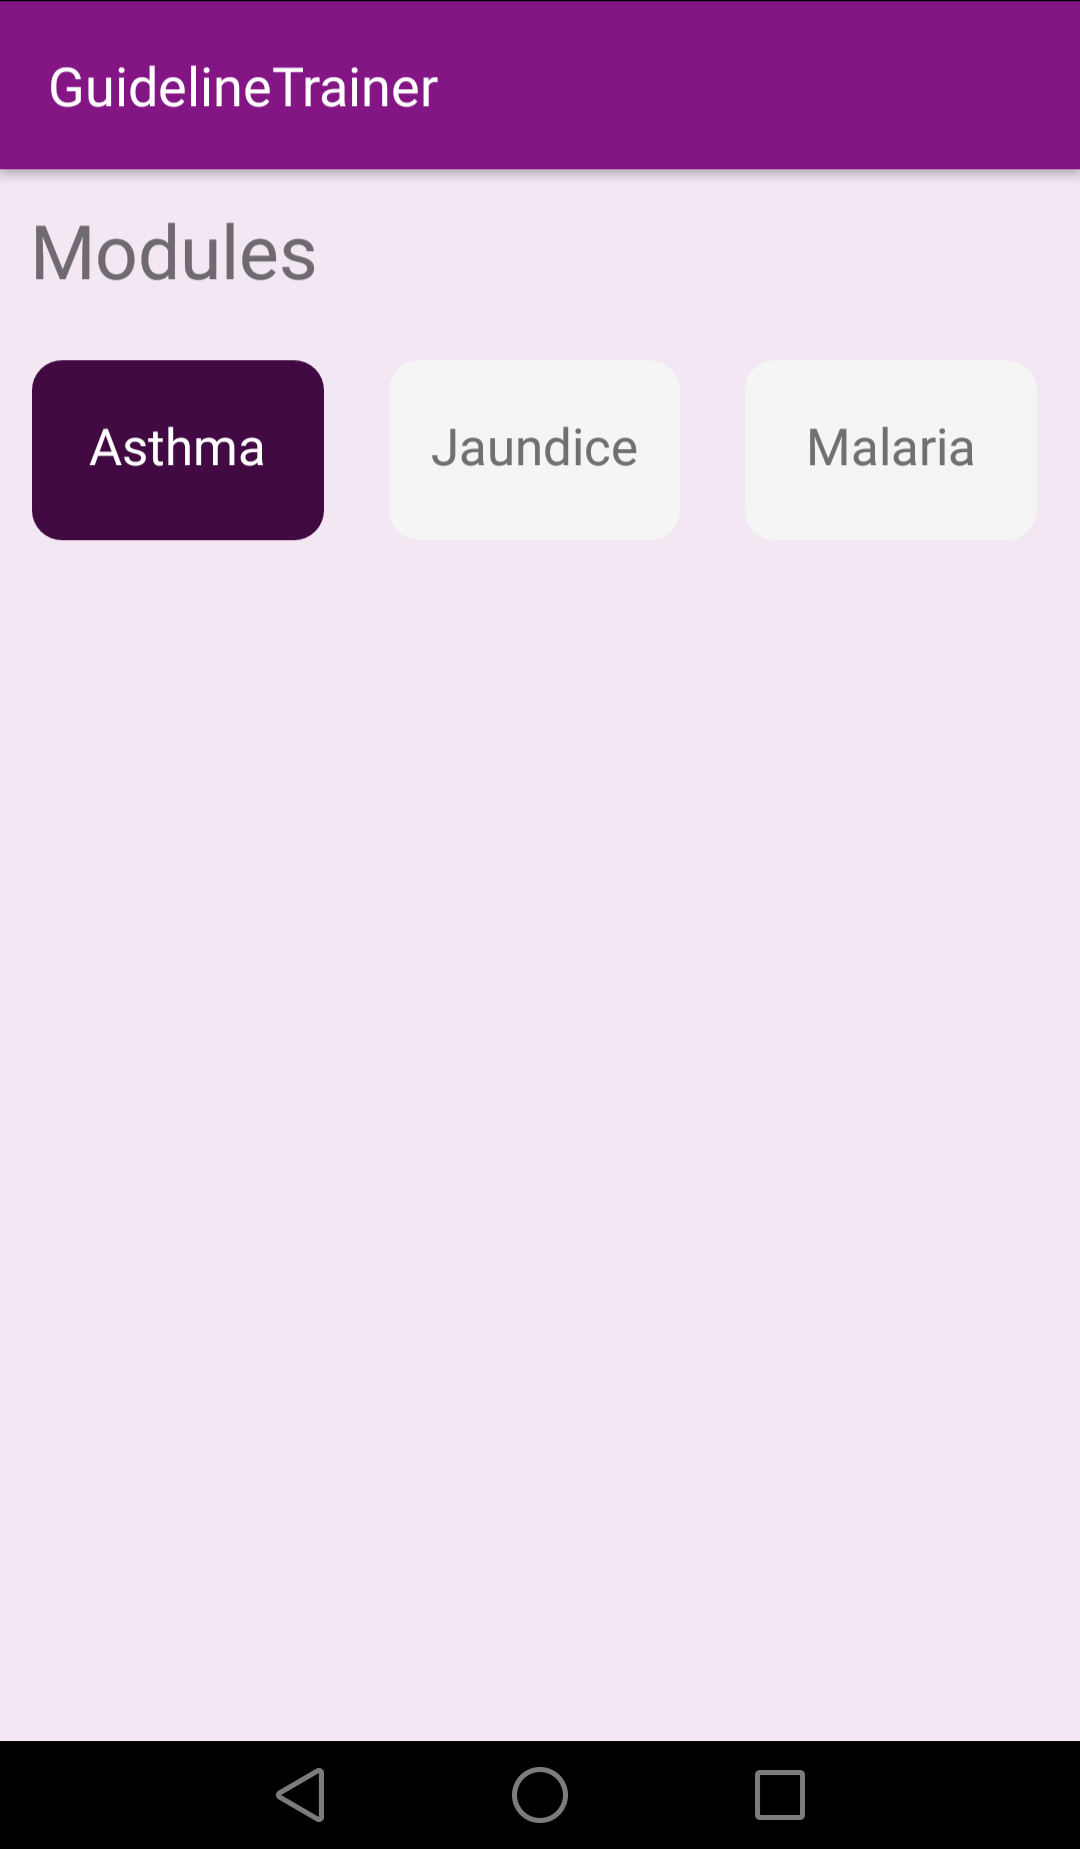
\includegraphics[scale=0.15]{ScreenshotMain}
	\caption {The entry screen where the student can choose between playing different quiz categories}
	\label{fig:ScreenshotMain}
\end{figure}

In \ref{fig:ScreenshotLearningMap} we get presented with the learning map from Dynamic Content Management \parencite{Eide2008}, and the student's position in the learning map. The boxes with the green background indicates the student's current position and which levels he will get questions from. The other background colours indicates which levels have been completed and which levels are uncompleted and locked. 

The student's position in the learning map is fetched from the database on the student's phone, and gets updated every time the student completes a quiz for this category. The database calls are asynchronously and loosely coupled using redux thunk \parencite{ReduxJS-thunk}, such that the web version would replace the database related functions with fetch related functions to for example do REST calls to a REST service. 

In the header we see a back arrow. This is React Native Navigation \parencite{Wix} which handles the navigation in the application, which makes it possible to click the arrow to go back and choose another quiz to play instead. This fulfils "Provide Clearly Marked Exits", which is one of the usability heuristics for user interface design given by Jakob Nielsen and Rolv Molich \parencite{Molich1990}.

\begin{figure}[h!]
	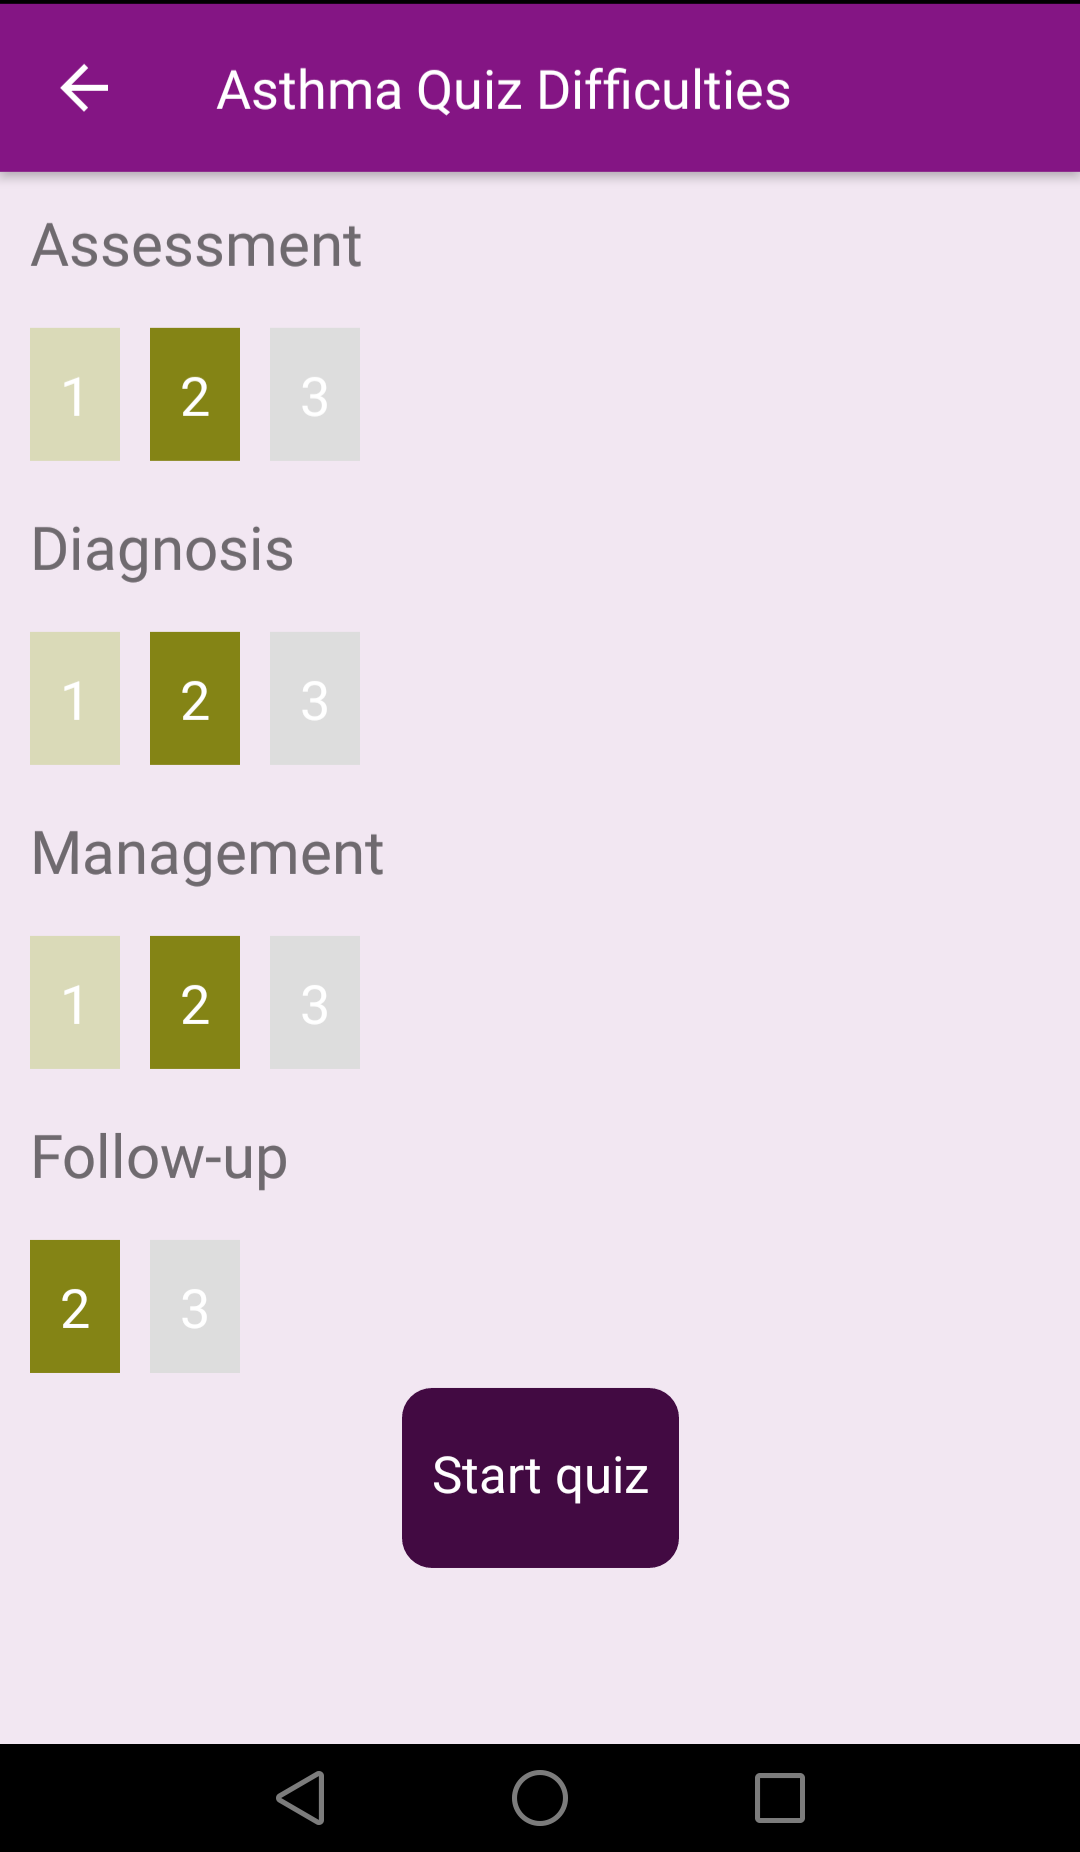
\includegraphics[scale=0.15]{ScreenshotLearningMap}
	\caption {The student is shown his position in the learning map. Completed, active and locked levels have all different colours}
	\label{fig:ScreenshotLearningMap}
\end{figure}

In \ref{fig:ScreenshotKarenAssessment} we are presented with a multiple choice question. The question is in the form of a scenario, where we go through the workflow model, where the first step is the assessment.  

The Game Engine holds a template and a reference to the entity instance graph which is being used with this template. The template contains tags which refers to vertices in the entity graph. The entity instance graph holds textual presentation of each vertex which is being printed into the template, which results in a neat and coherent text. 

The Game Engine an answer key, which is a tag pointing to one or more vertices in the entity instances. The Game Engine also holds hard coded distractions, where one of them matches the vertex/vertices which the answer key points to. Points and penalties are specified for each of the distractions in the Game Engine.

Here the student answers correctly, is awarded points and is being presented with an answer key explanation. The Game Engine holds the answer key explanation together with the question. 

The student can click on "next" any time he is ready to proceed to the next question.

\begin{figure}[h!]
	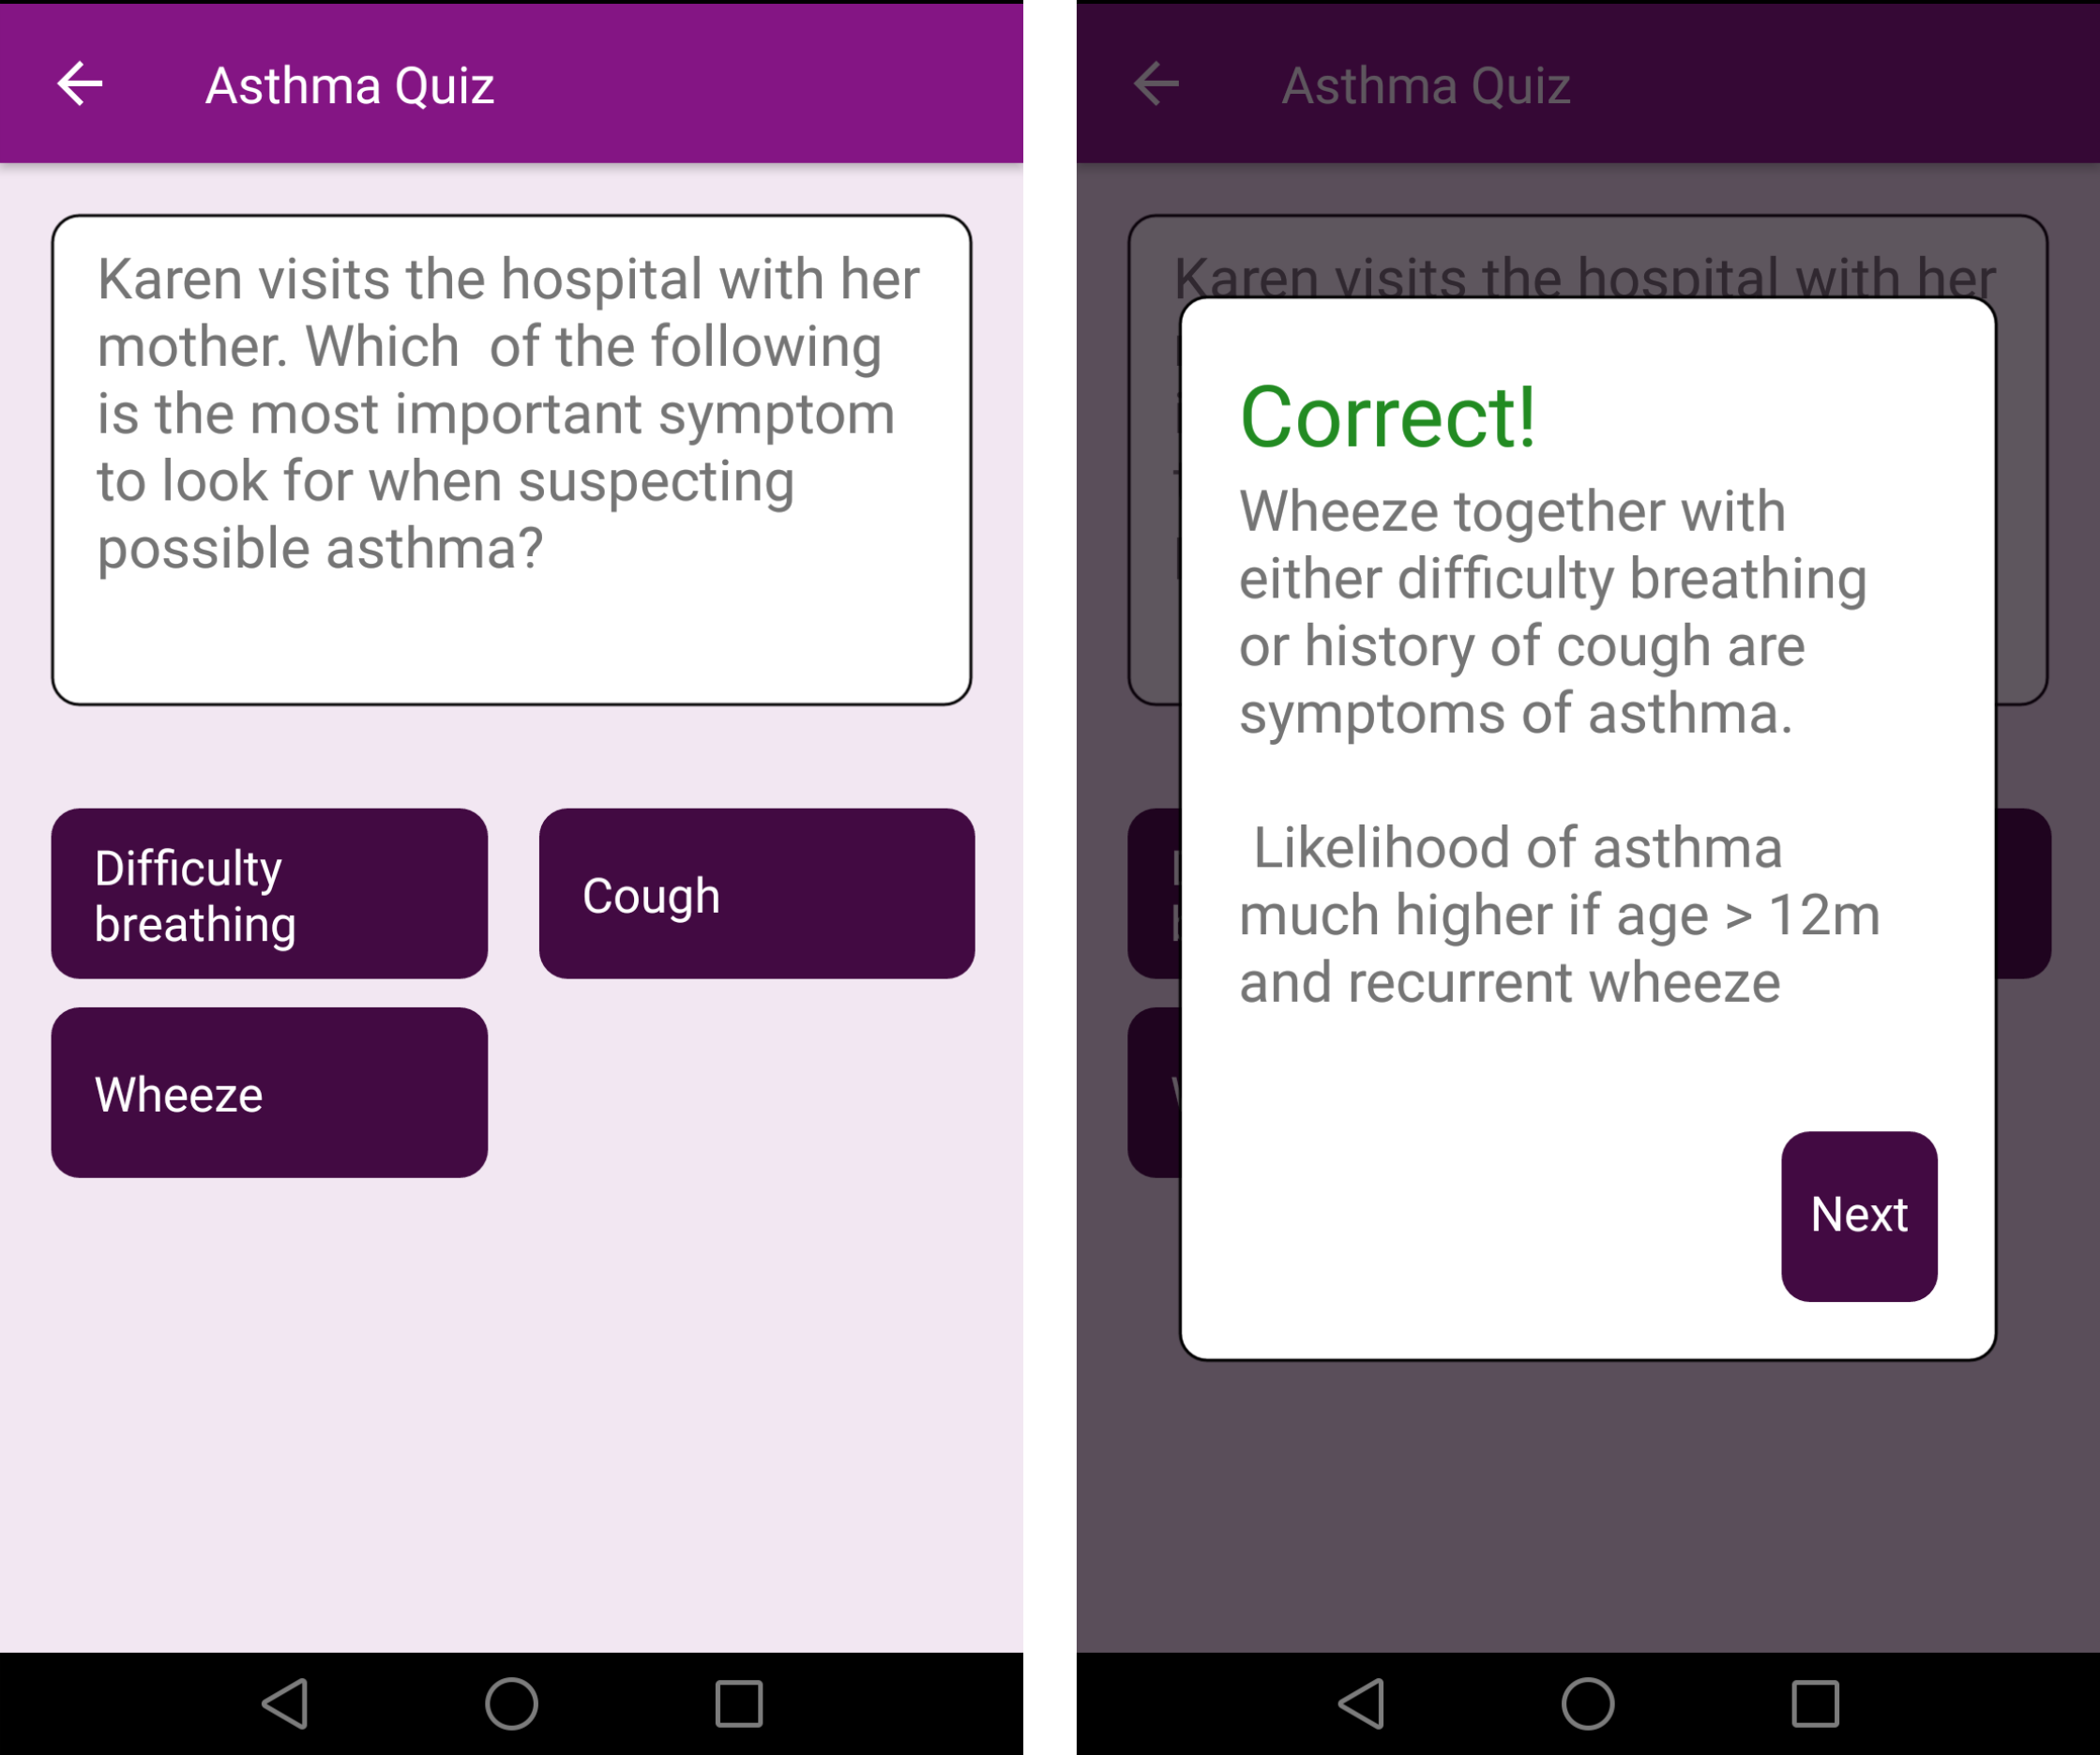
\includegraphics[scale=0.15]{ScreenshotKarenAssessment}
	\caption {The first question is an assessment question. Here answered correctly and an answer key explanation is given}
	\label{fig:ScreenshotKarenAssessment}
\end{figure}

In figure \ref{fig:ScreenshotKarenDiagnosis} we continue to the next step in the workflow model, the diagnosis. Here the student will be provided with symptoms which will determine the severity of the asthma.

\begin{figure}[h!]
	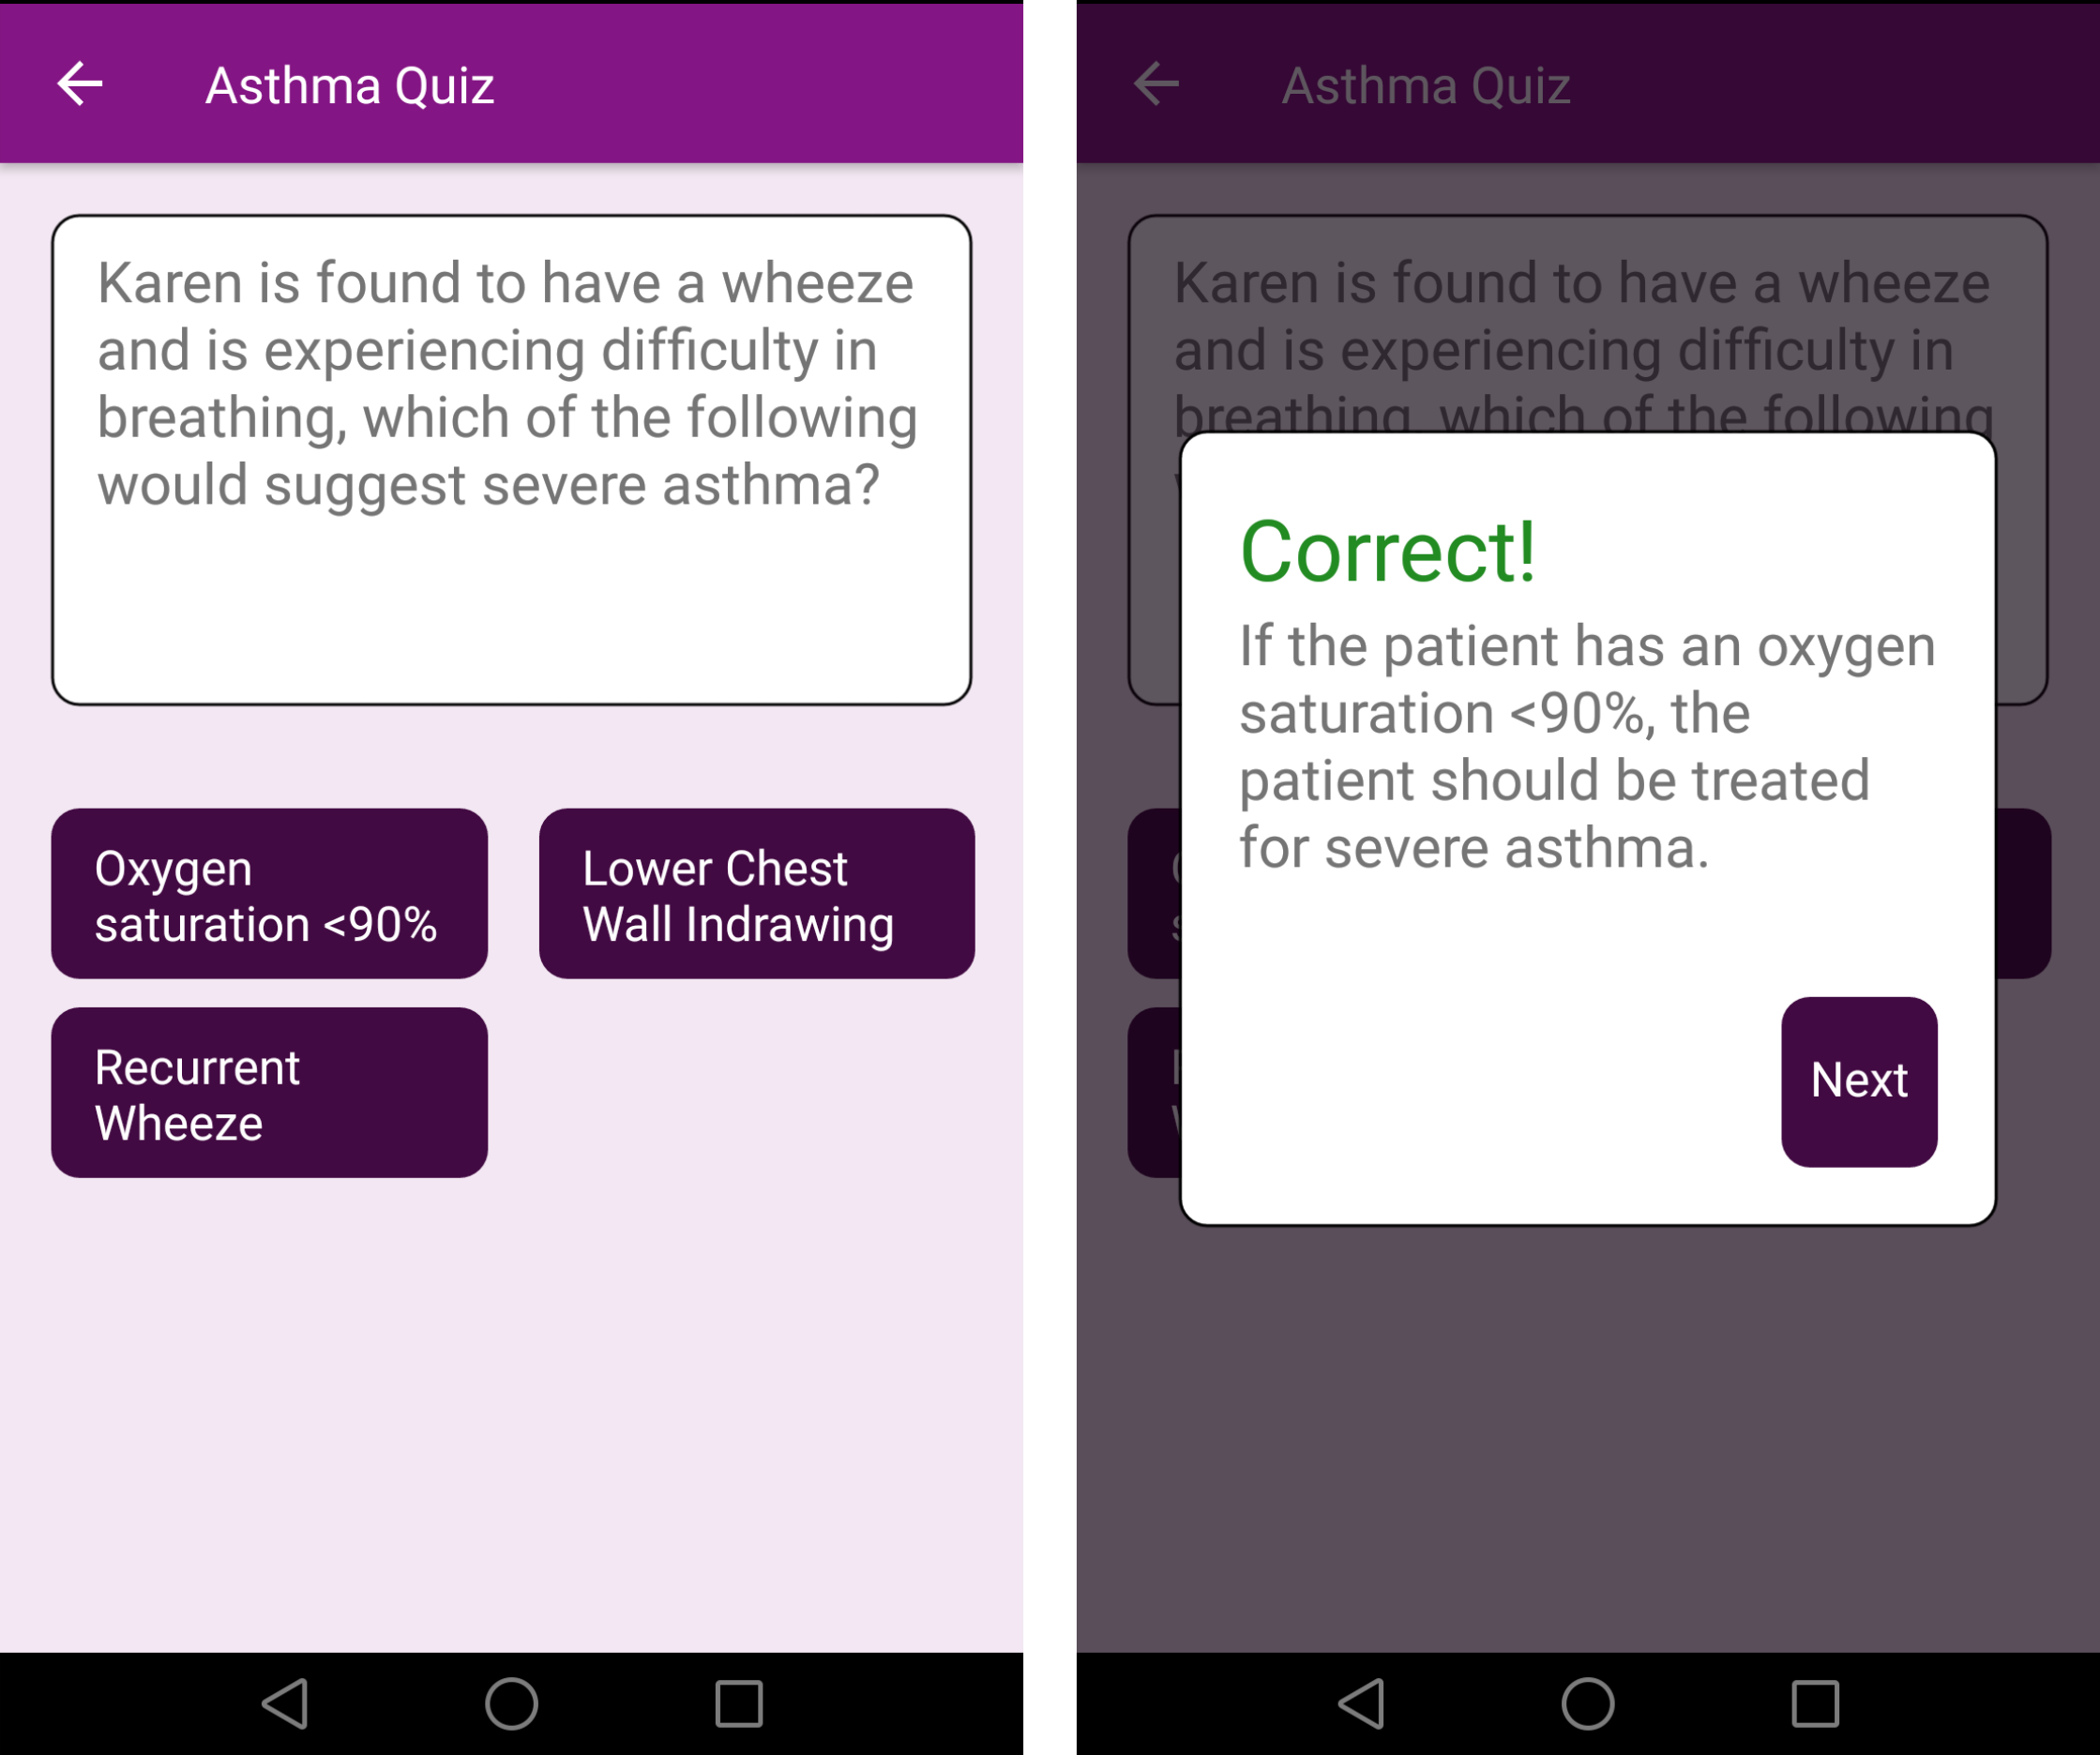
\includegraphics[scale=0.15]{ScreenshotKarenDiagnosis}
		\caption {The second question is for diagnosis}
		\label{fig:ScreenshotKarenDiagnosis}
\end{figure}

In figure \ref{fig:ScreenshotKarenManagement}, the student gets a question from the management part of the workflow model. Management can be admitting the patient to the hospital, medication administration or advise.
\begin{figure}[h!]
	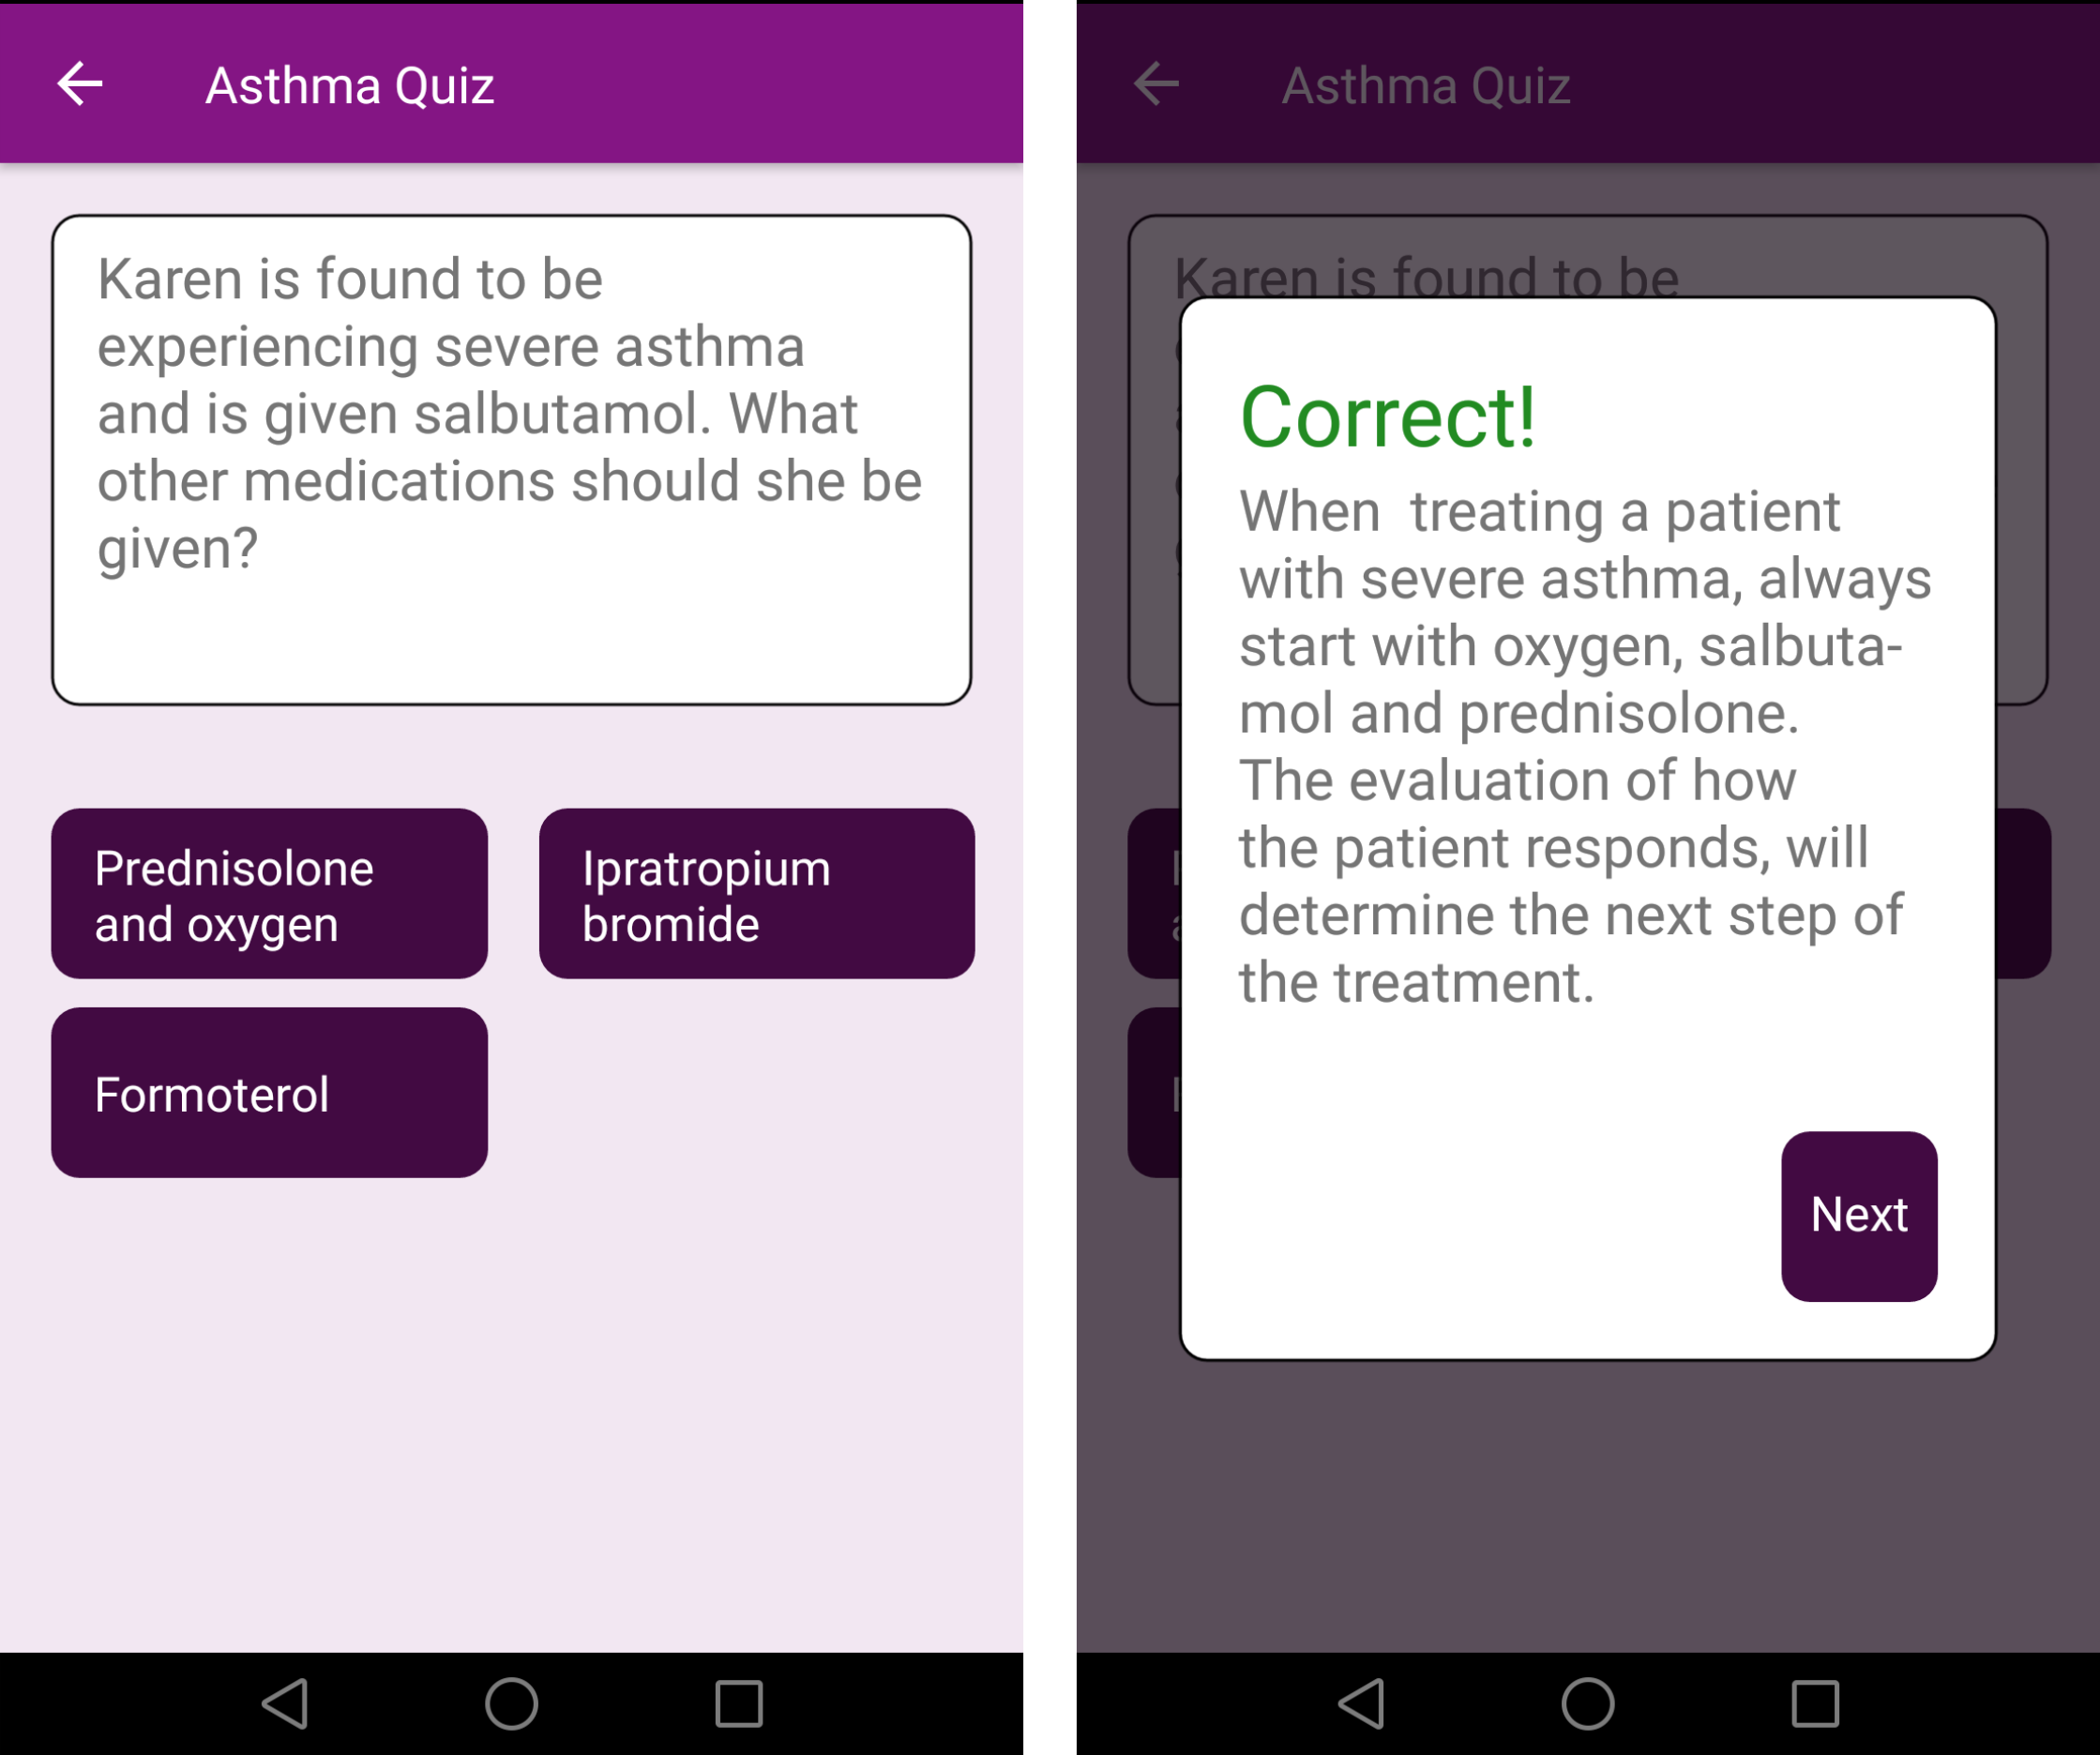
\includegraphics[scale=0.15]{ScreenshotKarenManagement}
	\caption {Third question is for management}
	\label{fig:ScreenshotKarenManagement}
\end{figure}

In figure \ref{fig:ScreenshotKarenFollowUp}, the patient has been through the initial treatment, and the student is asked on how to follow up the patient. Here the textbox in the screenshot is a bit small for the text, but the student has the possibility to scroll inside the textbox. The question is what is the maximum of days the patient can be on prednisolone.

Initially the student picks the wrong answer. The application displays a hint and a feedback, telling the student that this answer was wrong. The student is awarded with a penalty in points. As no further information is given rather than that the previous answer was wrong, the student is given the possibility to try again. If the student tries again, a wrong answer will give a further penalty. We have made sure that the penalty is much smaller than the reward, typically 10-20\% of the reward, trying to motivate the student to revise his answer. The student can try as many times that he would like, to get the answer correctly and collect the reward.

As we don't want to force the student to retry until correct, we have the option "learn more". When the student clicks on this button, he will be presented with the answer key explanation as well as the option to proceed to the next question. When the student decides to click on "learn more", he will miss out on the reward.

\begin{figure}[h!]
	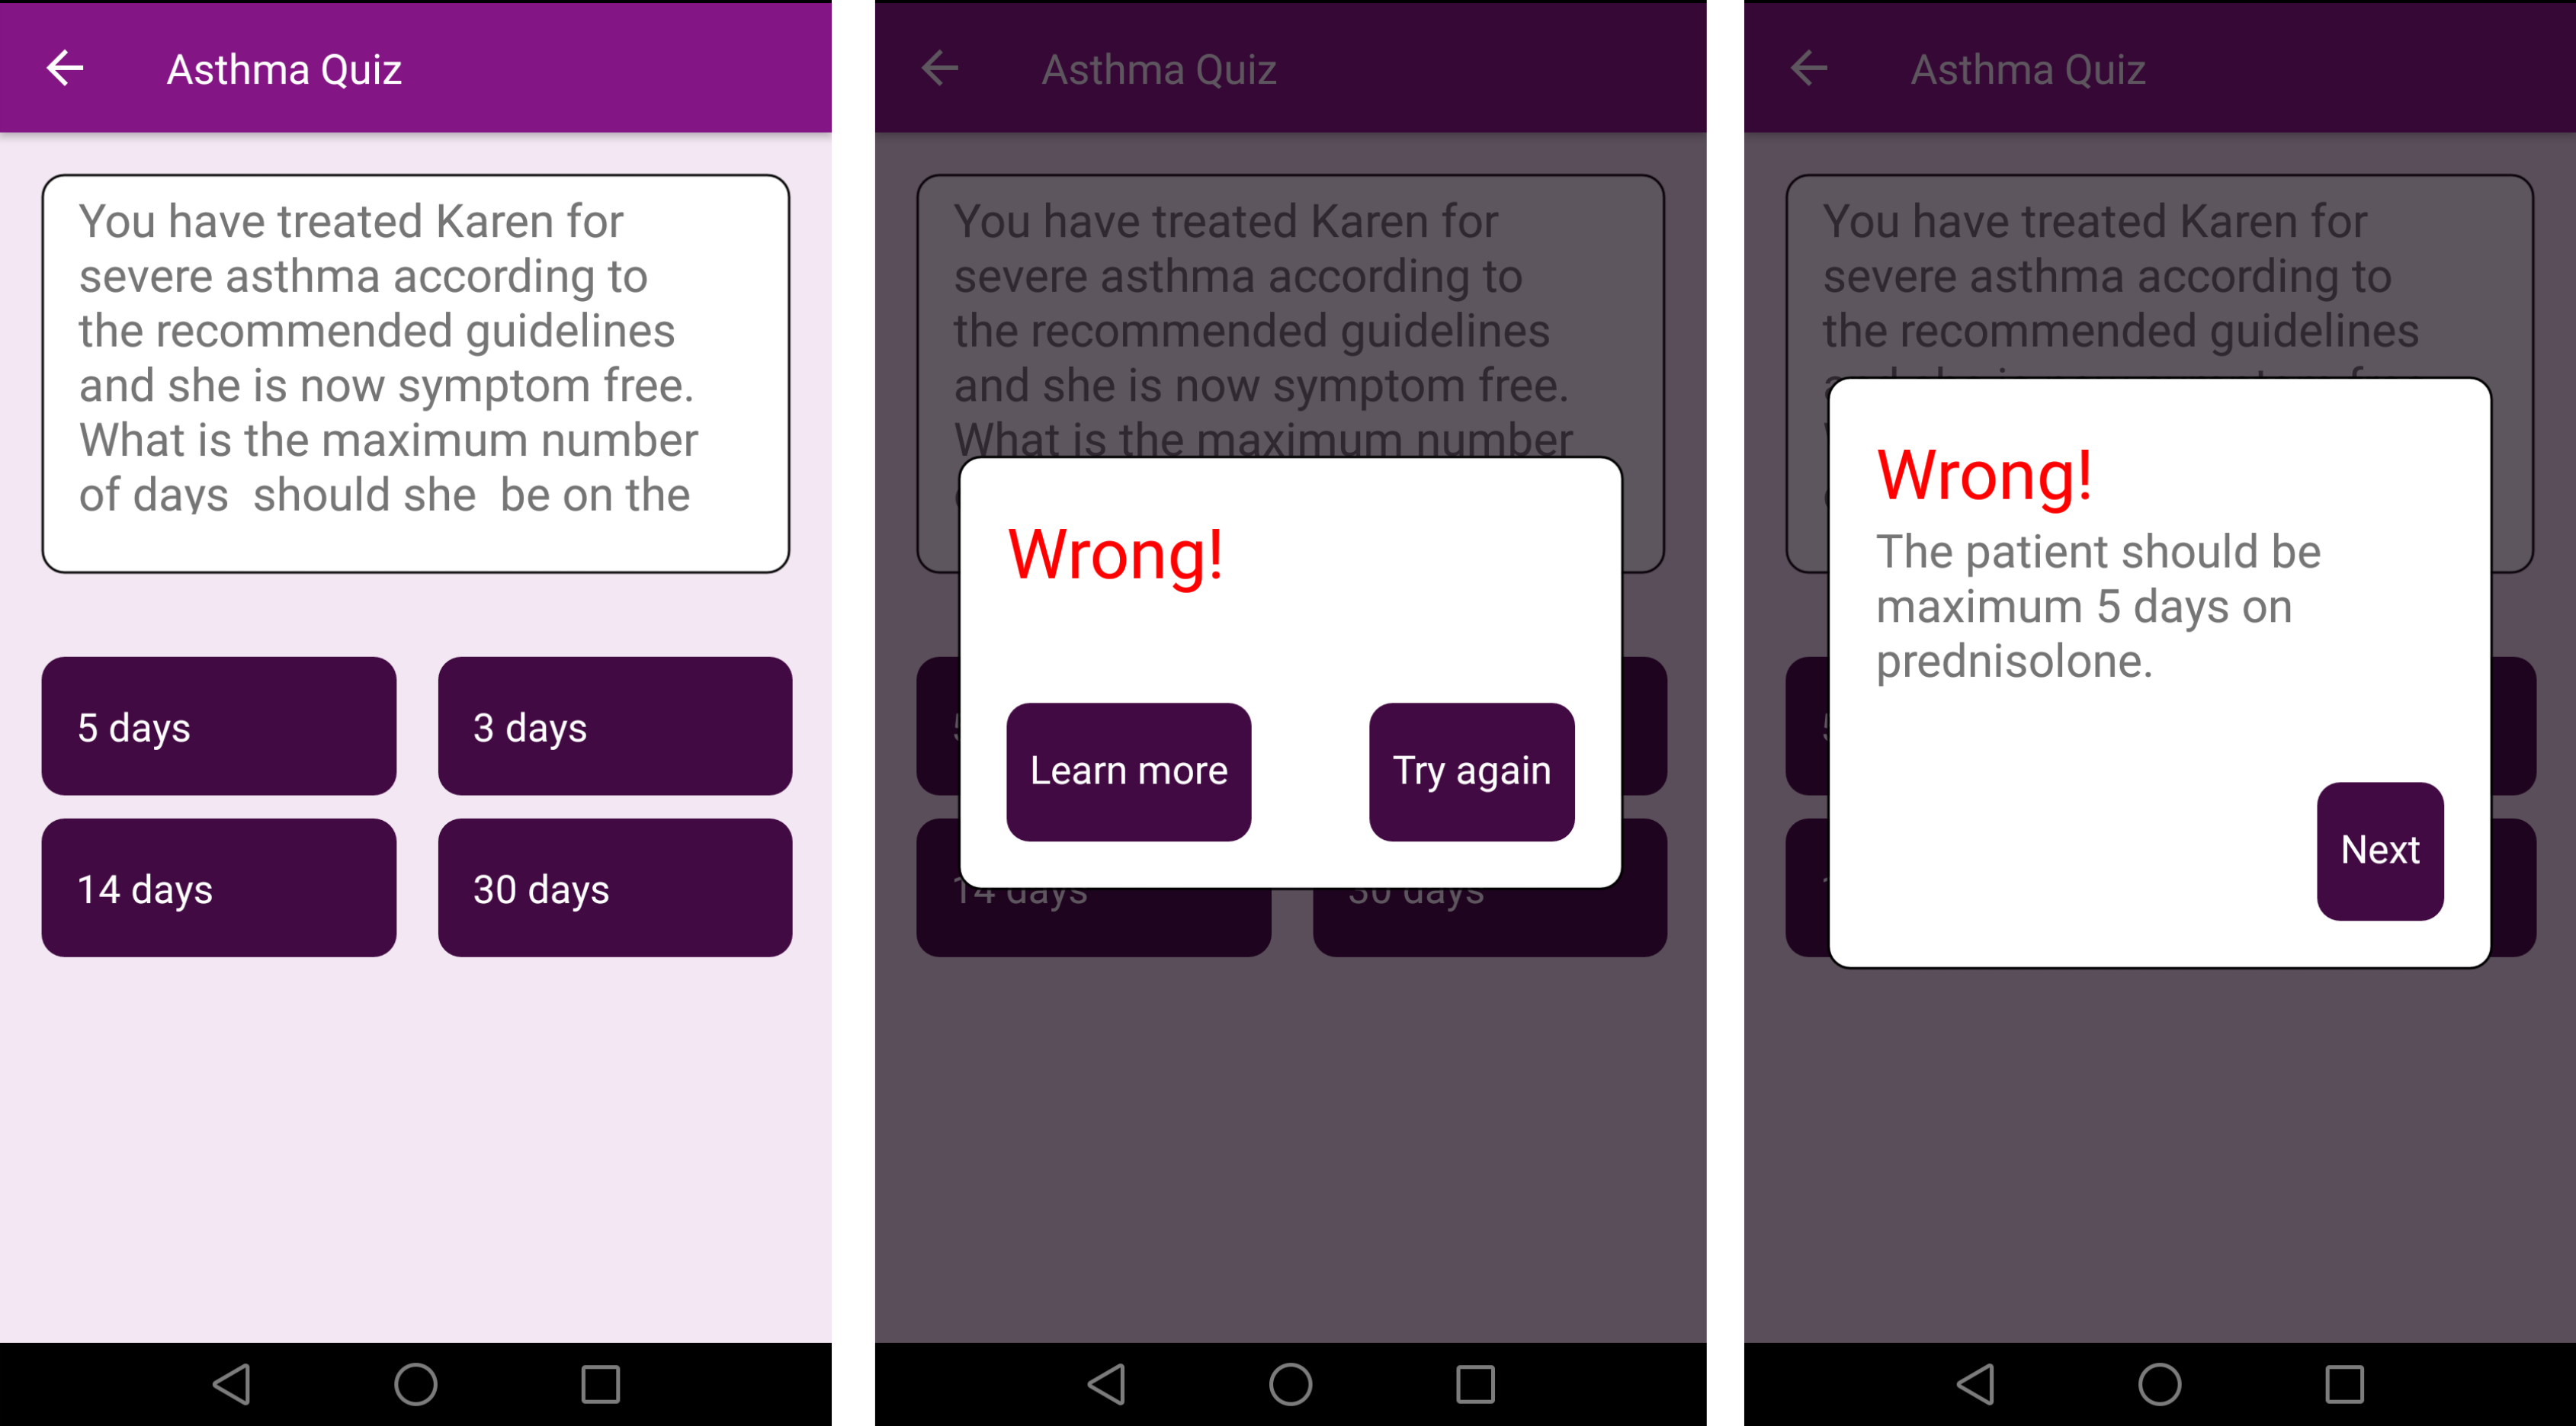
\includegraphics[scale=0.15]{ScreenshotKarenFollowUp}
	\caption {The fourth question is follow up. We answer incorrectly the first time. The answer key explanation is not shown, and we can choose to revise the question by clicking "try again". If we press "learn more", the answer key explanation is instead shown, and we continue to the next question}
	\label{fig:ScreenshotKarenFollowUp}
\end{figure}

When having answered follow-up, which is the last question in the workflow model and the scenario, the student will be presented with his updated position in the student map in figure \ref{fig:ScreenshotLearningMapUpdated}. Brown means previously unlocked levels. Grey means levels which are still locked and green means levels that have been unlocked after this game. If the student performs poorly, red boxes will appear. These boxes indicate that the current level has been locked, and that the student needs to complete quizzes at lower levels to repeat some of the more basic guideline content.

\begin{figure}[h!]
	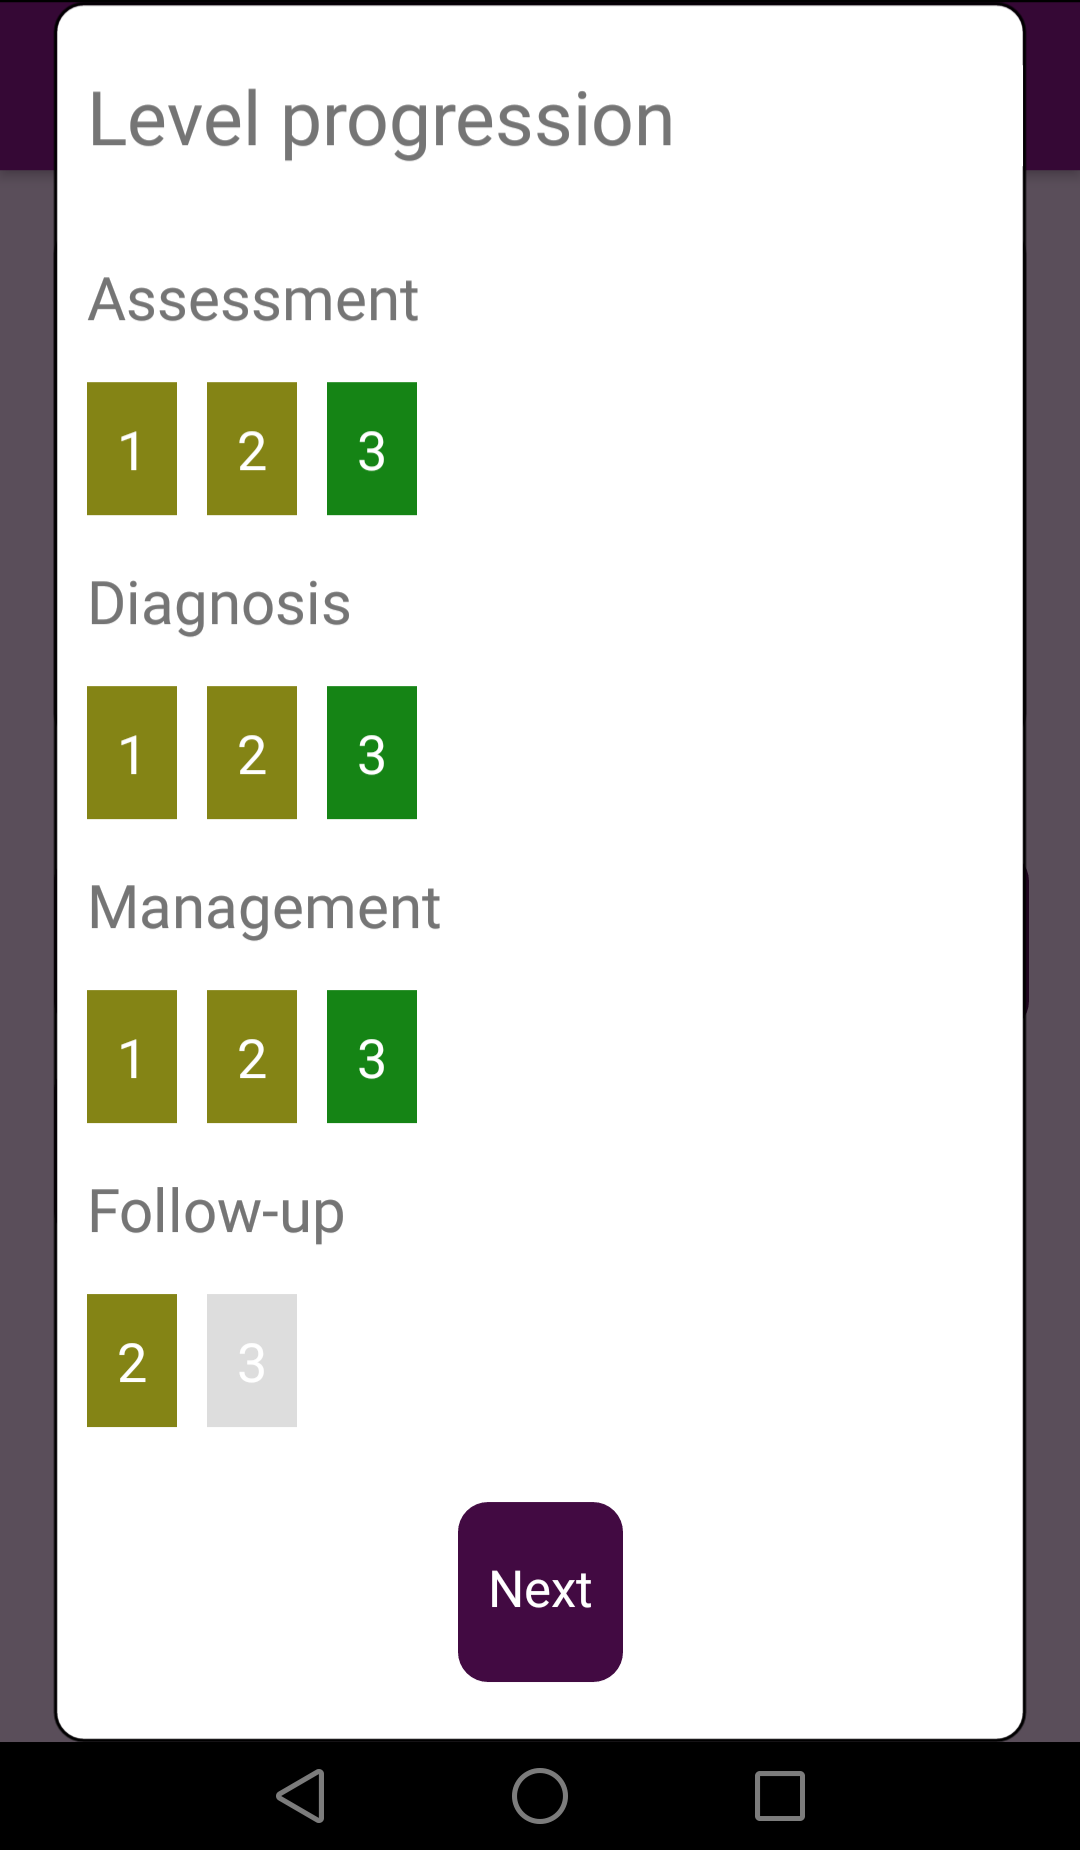
\includegraphics[scale=0.15]{ScreenshotLearningMapUpdated}
	\caption {After completing the quiz, we are shown the student's updated position in the learning map. The brown background shows levels which has been completed. Grey is the levels which are still unlocked. Green is that we have advanced to the next level. A red box would have indicated that we had performed poorly, the level would have been locked and we have to complete an easier level before we can play it again}
	\label{fig:ScreenshotLearningMapUpdated}
\end{figure}

The last screen in this game sequence is shown in figure \ref{fig:ScreenshotHighCharts}. The blue bars show our scores for the questions categorized according to the workflow model. The scores are for the current game we just played. The red lines show the scores needed to complete each category for the current level.

From the learning map and graph, we see that we completed the current level of assessment, diagnosis and management. We didn't complete follow-up, so the next time we play the asthma quiz we will only get questions from level 2 follow-up. The reason why the student won't get questions from assessment, diagnosis and management, is that we don't want to bore the student with continually asking the same questions that we know the student already knows the answers of.

The idea of the chart is to make the student motivated, when he sees his progress getting closer and closer to the red requirement line for every time he plays the asthma quiz at that level. Confirming that he learns more every time.

We used Highcharts \parencite{Highsoft} to display the interactive chart of the game scores and the scores required to complete each category.

\begin{figure}[h!]
	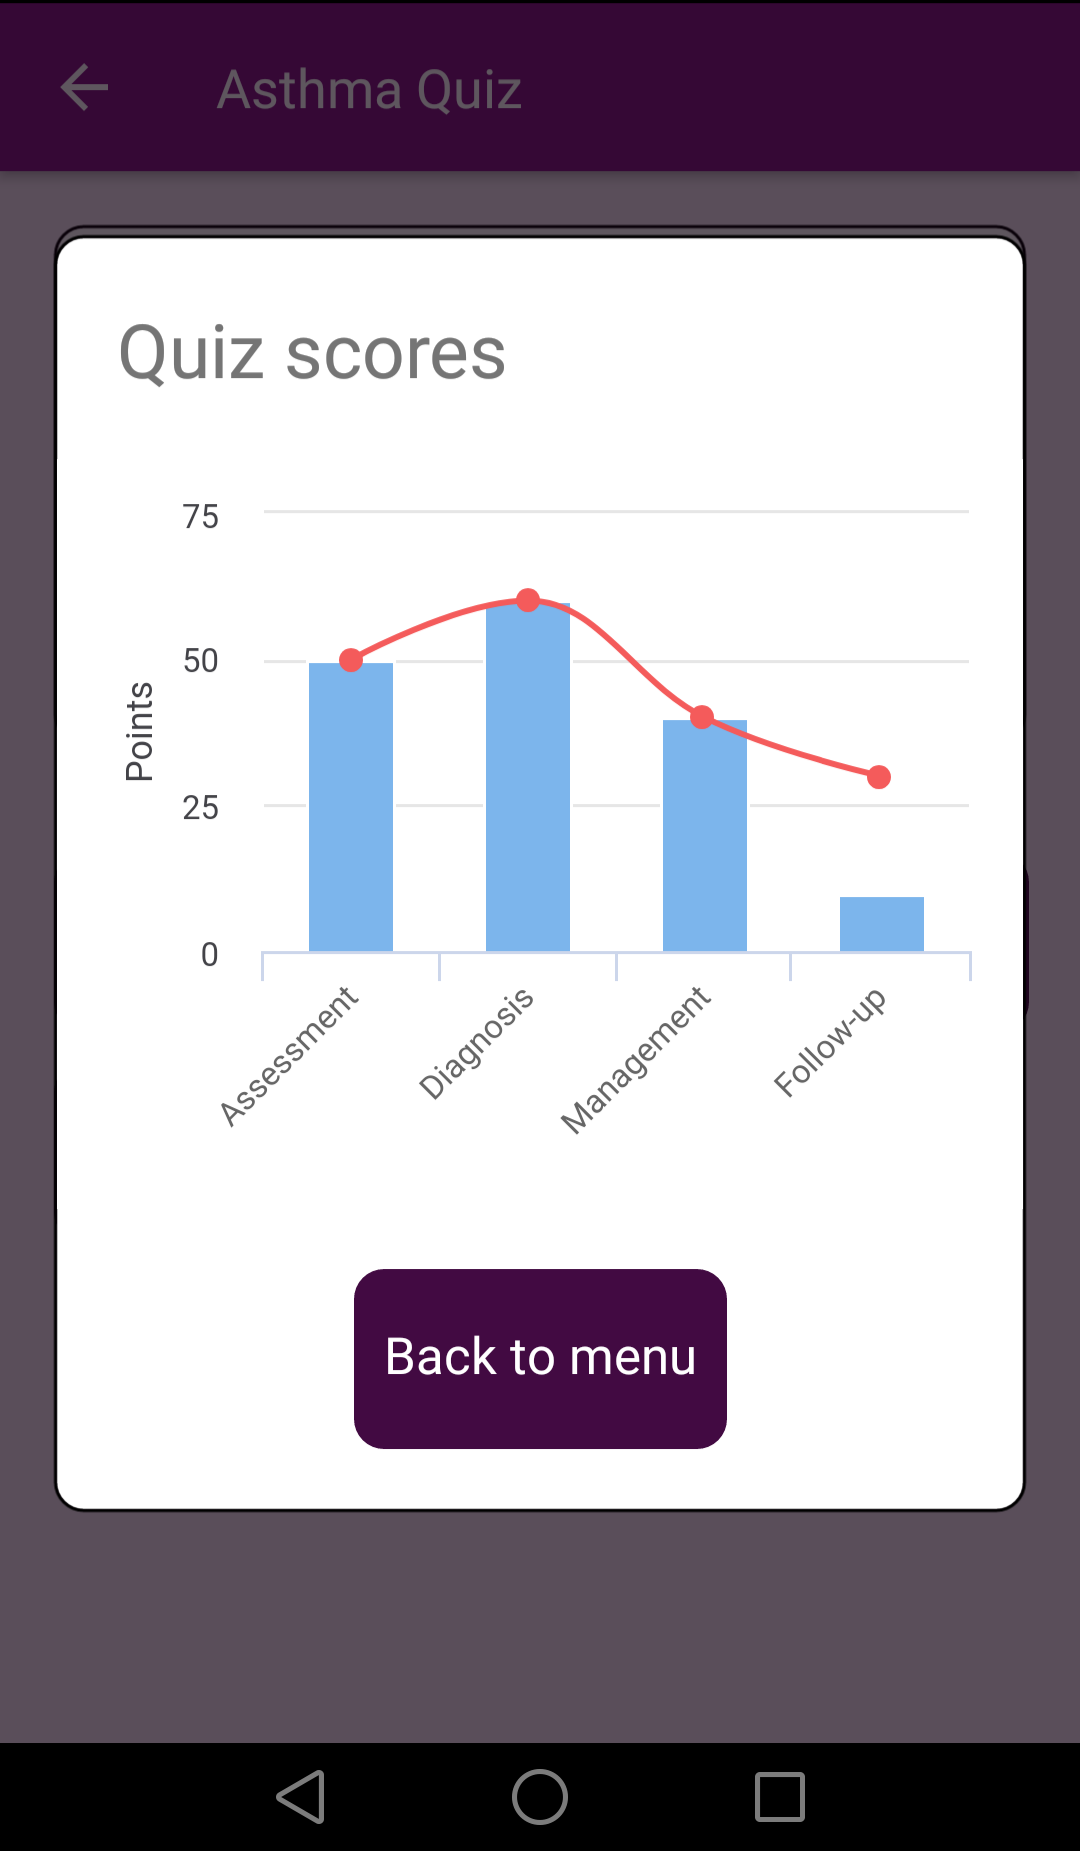
\includegraphics[scale=0.15]{ScreenshotHighCharts}
	\caption {The bars show our scores for the played game in the different parts of the clinical encounter. The red line shows the scores needed to complete this level}
	\label{fig:ScreenshotHighCharts}
\end{figure}

\section{Summary}
In this chapter we go through the mobile application by playing a game at level 2. We discuss the technologies which have been used, the user interface, intended user experience, the scoring system and some design choices. 

We show the student's performance in the current game with a chart. The chart represent the student's scores in different sections of the clinical encounter. A red line indicates the passing conditions at that difficulty level.

We see how the application adapts the difficulty to the knowledge progression of the student, by updating the student's position in the learning map.
	